\chapter{系统设计}
\label{design}

本系统一共由三部分组成。为了为用户提供一个具有真实触感的增强现实引擎,需要通过计算机和RGB-D摄像头结合起来进行物体识别和追踪,它们构成了后端引擎。同时,为了方便用户可以使用本系统进行编著和交互,前端基于Unity开发了一套应用程序,并且移植在Android移动端上。为了将用户编著数据和后端物体追踪数据进行传输,使用了网络通信。

\begin{figure}[!htp]
  \centering
  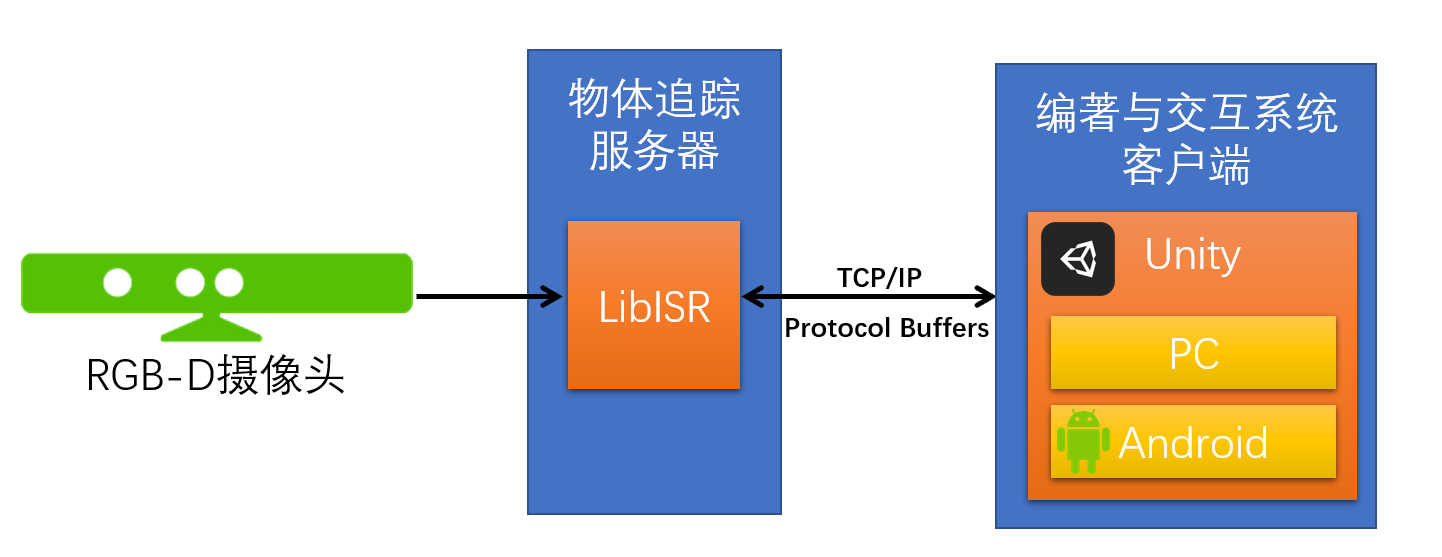
\includegraphics[width=12cm]{figure/TotalArc.png}
  \bicaption[系统架构图]
    {系统架构图}
    {The System Architecture Design}
 \label{fig:totalarc}
\end{figure}

综上所述,物体追踪引擎作为服务器,而编著和交互系统作为客户端,两者通过网络通信,本章节将会对这三部分的设计进行详细的介绍。

\section{服务器设计}

物体追踪引擎以LibISR为核心\cite{Ren_3DV_2014, star3d_iccv_2013},他的整体架构如图所示,其中只保留了比较核心以及在原程序上进行了一定修改的类。

\begin{figure}[!htp]
  \centering
  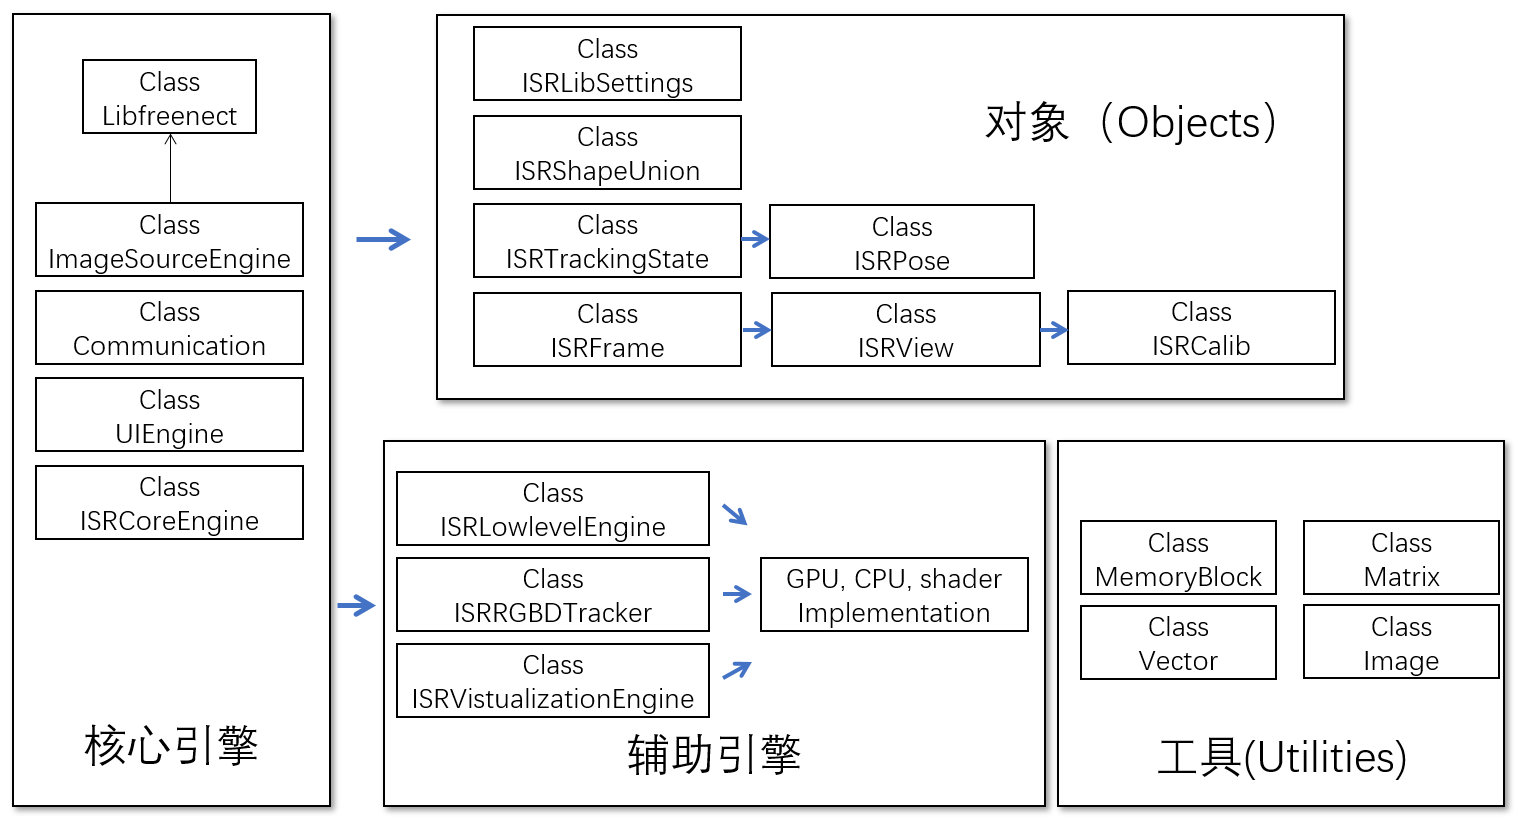
\includegraphics[width=12cm]{figure/LibArc.png}
  \bicaption[物体追踪架构图]
    {物体追踪架构图}
    {The Object Tracing Engine Architecture Design}
 \label{fig:labarc}
\end{figure}

整体架构共分为核心引擎、辅助引擎、对象、工具四部分。运行时,函数首先使用核心引擎进行初始化,包括使用的模型数据、追踪要求、标定数据等等,然后由负责网络、追踪、用户接口(UI)的引擎完成各自工作。这些工作涉及到的数据被封装为对象类。同时,LibISR还提供了一套自己的基础数据结构。

\subsection{对象}

对象是一些不包含业务逻辑,只负责将数据进行封装、整合、处理的类。首先对这些对象进行介绍,可以方便之后的讲述。

\begin{itemize}
    \item \textbf{ISRCalib}
用于储存标定数据,包括深度摄像头和彩色摄像头的内参、外参,以及单质性矩阵,这些标定数据又由单独的对象类进行储存。相机本身的参数通过读取标定数据文件进行读取,而单质性矩阵则通过计算上述变量得出。
    
    \item \textbf{ISRPose}
储存物体的追踪结果,追踪结果由物体的旋转矩阵和位移向量组合起来的4x4矩阵。
    
    \item \textbf{ISRView}
储存相机读取的图像以及经过处理的中间数据。包括原始的彩色图像、深度图像,以及将彩色图映射到深度图的图像等。

    \item \textbf{ISRFrame}
储存了RGB-D图片的中间处理结果,例如点云、碰撞图、ISRView。
    
    \item \textbf{ISRTracingState}
主要用于多物体追踪,保存所有物体的ISRPose,被用于计算代价函数。

    \item \textbf{ISRShapeUnion}
主要用于多物体追踪,保存由所有物体的模型组合而成的shape union。

    \item \textbf{ISRLibSettings}
保存项目的相关设置,包括是否使用GPU加速,是否追踪一种模型等。
\end{itemize}

\subsection{核心引擎}

核心引擎是暴露给用户的接口,负责启动物体追踪、与硬件、网络、用户交互等核心功能。用户可以通过创建核心引擎的对象,从而实现物体追踪的功能。

\begin{itemize}
    \item \textbf{ImageSourceEngine}
该类是一个纯虚类,他负责连接硬件(摄像头),将读取到的数据进行格式转换、适配,保存在ISRView中,并将指针提供给其他引擎以供图片读取。
    
    \item \textbf{Communication}
该类作为服务器,负责开启数据传输服务,等待前端用户输入并进行处理。
    
    \item \textbf{UIEngine}
该类主要负责通过OpenGL实现用户前端,将追踪的原始RGB图像、深度图像、追踪结果进行显示。并且通过glut的接口,获得用户输入,包括开始、重置、暂停、截屏等等。

    \item \textbf{ISRCoreEngine}
它是物体追踪的核心引擎。在每一帧都会运行,将获取的图片进行处理,调用ISRRGBDTracker对象进行计算,获得物体位置后更新ISRTrackingState等对象,并且调用ISRVisualisationEngine将追踪的结果使用OpenGL进行可视化,之后由UIEngine进行显示。

\end{itemize}

\subsection{辅助引擎}

辅助引擎是辅助ISRCoreEngine进行工作的类,包含部分业务逻辑。这三类都是纯虚类,会根据硬件情况采用C++代码或CUDA\cite{CUDARef}代码的实现。

\begin{itemize}
    \item \textbf{ISRLowlevelEngine}
该类负责融合RGBD图像、应用滤波、获得bounding box、根据RGBD图像获得点云数据等功能
    
    \item \textbf{ISRRGBDTracker}
用于进行物体追踪的计算,包括标记前后景像素、计算代价函数、计算Jacobian矩阵用于最小化代价函数等功能的实现。
    
    \item \textbf{ISRVisualisationEngine}
用于中间数据的可视化,以及最终结果的渲染,包括渲染被追踪的物体、渲染深度图、渲染SDF模型应用结果等。
\end{itemize}

\subsection{工具}

LibISR基于C++基本的数据结构进行了进一步的封装,实现了向量(vector)、矩阵(matrix)、图像(image)、数据块(memory block)等数据结构。向量和矩阵再提供基本运算的基础上,还提供了针对于实际需求的成员变量名字,例如Vector3具有r,g,b三个成员,或x,y,z三个成员。此外,图像还提供了保存为文件的函数。数据块则为了统一管理在CPU和GPU进行转换的数据。